\chapter{Parallel IDS Design on GPUs}
\vspace{\topsep} 
\section{Overview of Parallelism Approaches}
There are two types of parallelism employed to speed up packet processing on the GPU as shown in Fig. ~\ref{fig:thread-level} and Fig. ~\ref{fig:block-level}.
\begin{figure}[H]
	\centering
	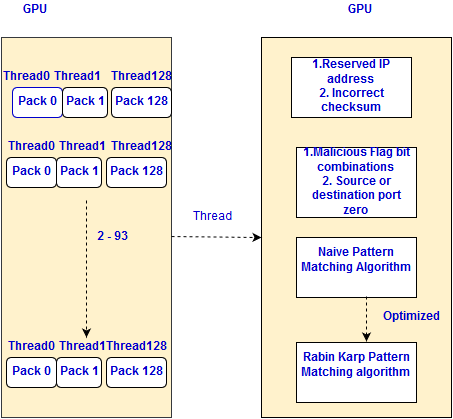
\includegraphics[width=10cm]{threadlevel.png}
	\caption{Thread-level parallelism}
	\label{fig:thread-level}
\end{figure}
\squeezeup
\subsection{Thread-Level Parallelism}
In thread-level parallelism, each packet was analyzed by one thread. The kernel was launched with 260 blocks of 256 threads each. A thread executed both header checking and pattern matching. The code was optimized to use shared memory. Signatures are stored in global memory. In the naive pattern-matching algorithm, each thread accesses global memory N times, where N is the number of patterns multiplied by the maximum pattern length. The time taken to access data from global memory is approximately 200 to 300 cycles \cite{bib14}. \\ In order to decrease the amount of global memory accesses, the Rabin-Karp algorithm was developed. In the Rabin-Karp algorithm, each thread accesses global memory only M times, where M is the total number of patterns. 
\subsection{Block-Level Parallelism}
In block-level parallelism, a group of 256 threads cooperatively process each packet. The entire block of threads cooperatively execute header checking and pattern matching on a single packet. In this approach, warp divergences was encountered due to if conditions. To eliminate warp divergence, the code was modified such that threads in different warps execute different if conditions. For example, threads in warp 1 execute the IP rules, threads in warp 2 execute the TCP rules and threads in the remaining warp execute pattern matching. 

\begin{figure}[H]
	\centering
	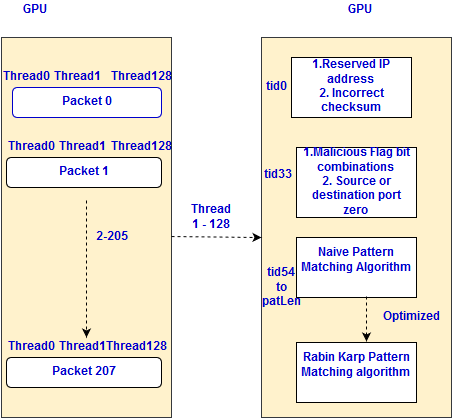
\includegraphics[width=10cm]{blocklevel.png}
	\caption{Block-level parallelism}
	\label{fig:block-level}
\end{figure}
\squeezeup

\section{Header Checking}
An attacker may send crafted packets to a computer in order to consume all of its resources, such that it cannot service any other request. To identify crafted packets, header checking evaluates the validity of the header part of a given packet. The headers of the packets were analyzed by applying the following rules on them.

The rules are:
\begin{enumerate}[leftmargin=*]
	\item
	Check if the IP address of the packet is in the private address range, because there can be no computer on the Internet whose IP address is in this range.
	\item
	Check if the flag bits in the TCP header are crafted or check if the reserved bits are set. Consider as an example that, it is not possible to have a combination of the SYN and FIN bit set.
	\item
	Check if the acknowledgment bit is set and the acknowledgment number is zero. Check if the source or destination port is zero for a TCP packet.
	\item
	Check if the IPv4 checksum was tampered while in transit.
	If any of the above rules match, the packet is discarded from further processing.
\end{enumerate}
\vspace{\topsep}
When a packet passes all the above rules, pattern-matching algorithms are applied on the packet. Otherwise, an administrator is notified. Currently, there are four rules for header checking, but the IDS can be easily scaled to cover more rules.

\section{Parallel Pattern-Matching Algorithms using CUDA}
\vspace{\topsep}
\subsection{Rabin-Karp Algorithm}
The single-pattern Rabin-Karp algorithm was modified to obtain the multi-pattern-matching algorithm. In the multi-pattern-matching version, the patterns are represented by a two-dimensional array. In order to copy the two-dimensional array to the GPU, the array is flattened to a one-dimensional array, which is then copied to the GPU. 
Each thread compares the hash code of every pattern against the payload starting from the position that corresponds to its thread index.\\ Multiple iterations are run by each thread, corresponding to the number of patterns. As shown in Fig. ~\ref{fig:multi rabin-karp}, all of the threads with a thread index above 53 perform pattern matching. Each thread iterates over all patterns and applies the Rabin-Karp algorithm to each pattern. Therefore, the execution time is very long. Thus, this algorithm is not suitable for multiple pattern matching.

\begin{figure}[H]
	\begin{lstlisting}
	/*Rabin Karp Multi-pattern string matching implementation*/
	if(threadIdx.x >= 54) {
	GPU_results[0].num_strings = const_num_strings;
	
	for(int i=0;i<const_num_strings;i++) {
	int patLen = const_indexes[2*i+1] - const_indexes[2*i];
	//This condition checks if the pattern length is < packet length
	if(threadIdx.x<=256-patLen) {
	int hy,j;
	for(hy=j=0;j<patLen;j++) {
	if((j+threadIdx.x) >= 256) goto B;
	hy = (hy * 256 + elements[j+threadIdx.x].packet) % 997;
	}
	if(hy == const_patHash[i] && memCmpDev<T>(elements,const_pattern,const_indexes,i,threadIdx.x,patLen) == 0)  {
	GPU_results[blockIdx.x].maliciousPayload = 1;
	GPU_results[blockIdx.x].signatureNumber = i; 
	d_result[i]=1;
	} 
	}
	}		
	\end{lstlisting}
	\caption{Parallel implementation of the Rabin-Karp algorithm}
	\label{fig:multi rabin-karp}
\end{figure}
\squeezeup

\subsection{Aho-Corasick Algorithm}
Each thread searches for multiple patterns starting from its thread index. Each thread uses the goto table present in global memory to advance to the next state based on the character at its position. Then, each thread checks the output array to see if there are any virus patterns at this position and adds the index of the pattern to the result if there was a match. Since each thread starts at a particular byte of the input text, the failure table was not used in the GPU-version algorithm. Thus, the failure-less Aho-Corasick algorithm was implemented \cite{bib20}, as shown in Fig. ~\ref{fig:multi aho-cor}.

\begin{figure}[H]
	\begin{lstlisting}
	//Aho Corasick Algorithm
	if(threadIdx.x>=54)
{
int pos=threadIdx.x;
char ch = elements[pos++].packet;
int chint = ch & 0x000000FF; 
int nextState = stateszero[chint];
if(nextState!=0) {
if(d_output[nextState] > 0) result[blockIdx.x] = d_output[nextState];
while(nextState!=0 && pos<256) {
ch = elements[pos++].packet;
chint = ch & 0x000000FF;
nextState = gotofn[nextState*256 + chint];
if(d_output[nextState] > 0) result[blockIdx.x] = d_output[nextState];
}
}
}
	\end{lstlisting}
	\caption{Parallel implementation of the Aho-Corasick algorithm}
	\label{fig:multi aho-cor}
\end{figure}
\squeezeup

\subsection{Wu-Manber Algorithm}
Each thread searches for multiple patterns starting from its thread index. The threads compute the hash value of the suffix from its (position + m-1) array index, where m is the minimum pattern length up to three characters backward, as shown in Fig. ~\ref{fig:wumanstep1}, and check if the shift value from the shift table is zero. 

If the value of shift is zero, then the hash value of the prefix starting from its thread index up to two characters is calculated and searched in the prefix table to check if it exists as shown in Fig. ~\ref{fig:wumanstep2}. 

\begin{figure}[H]
	\begin{lstlisting}
	//Each thread starts searching from its thread Id. elements array contains the 256 byte packet //and is stored in shared memory.
	unsigned int hash1, hash2;
	if(threadIdx.x >= 54 + m-1) {
	hash1 = elements[threadIdx.x - 2].packet & 0x000000FF; //bitwise & used because to avoid two complement negative numbers
	hash1 <<= 2;
	hash1 += elements[threadIdx.x - 1].packet & 0x000000FF;
	hash1 <<= 2;
	hash1 += elements[threadIdx.x].packet & 0x000000FF;
	int shift = d_SHIFT[hash1];
	\end{lstlisting}
	\caption{Calculating the hash value of the suffix}
	\label{fig:wumanstep1}
\end{figure}
\squeezeup

The patterns located at a particular prefix are compared with the text by a memory compare operation. If there is a match, the pattern index is added to the resulting structure. Since each thread starts from a particular byte and all indexes of the text are handled by a thread, the threads need not shift forward and continue the search again. Therefore, each thread executes the algorithm only once.

\begin{figure}[H]
	\begin{lstlisting}
if (shift == 0) {
hash2 = elements[threadIdx.x - m + 1].packet & 0x000000FF;
hash2 <<= 2;
hash2 += elements[threadIdx.x - m + 2].packet & 0x000000FF;

//For every pattern with the same suffix as the text
for (int i = 0; i < d_PREFIX_size[hash1]; i++) {	
//If the prefix of the pattern matches that of the text
if (hash2 == d_PREFIX_value[hash1 * prefixPitch + i]) {
int patIndex = d_PREFIX_index[hash1* prefixPitch + i];
int starttxt = threadIdx.x - m + 1 + 2;
int startpat = d_stridx[2*patIndex] + 2;
int endpat = d_stridx[2*patIndex+1];

//memcmp implementation
while(elements[starttxt].packet!='\0' && startpat < endpat) {
if(elements[starttxt++].packet!=d_pattern[startpat++]) return;
}
if(startpat >= endpat) { 
printf("The pattern exists %d\n", patIndex);
GPU_results[blockIdx.x].maliciousPayload = 1;
result[blockIdx.x] = patIndex;
}
}
	\end{lstlisting}
	\caption{Pattern is searched based on the hash value of the prefix}
	\label{fig:wumanstep2}
\end{figure}
\squeezeup

\section{Utilization of Pinned Memory}
Two different versions of the three algorithms were developed. One version used pinned memory to transfer data from the CPU to the GPU and another used non-pinned memory. Fig. ~\ref{fig:nonpinnedmemory} illustrates a case in which data are transferred without using pinned memory. In this case, memory should be allocated using the cudaMalloc() function and then the contents should be copied from host to device memory using the cudaMemcpy() function. 

\begin{figure}[H]
	\begin{lstlisting}
	//Allocate host side memory
	int * result = (int*)malloc(N *sizeof(int));
	
	//allocate device side memory
	cudaAssert(cudaMallocPitch(&d_gotofn,&pitch,chars * sizeof(int),states));
	
	//copy from host memory to device memory
	cudaAssert(cudaMemcpy2D(d_gotofn,pitch,gotofn,chars * sizeof(int),chars * sizeof(int),states,cudaMemcpyHostToDevice));
	
	//copy result from device memory to host memory
	cudaAssert(cudaMemcpy(result,d_result,N *sizeof (int),cudaMemcpyDeviceToHost));
	\end{lstlisting}
	\caption{Using non-pinned memory for data transfer}
	\label{fig:nonpinnedmemory}
\end{figure}
\squeezeup

Pinned memory should be allocated using the cudaHostAlloc() function and a pointer to the allocated memory should be passed to the GPU as shown in Fig. ~\ref{fig:pinnedmemory}. The host and the device can access pinned memory. Hence, a memory copy is not required to transfer data back and forth between the device and the host.

\begin{figure}[H]
	\begin{lstlisting}
	//Allocate Pinned Memory
	cudaAssert(cudaHostAlloc((void**) &array, states * 256 * sizeof(int), cudaHostAllocMapped));
	cudaAssert(cudaHostAlloc((void**) &result, N * sizeof(int), cudaHostAllocMapped));
	
	//Getting the device pointer for the pinned memory
	cudaAssert(cudaHostGetDevicePointer(&d_gotofn, array, 0));
	cudaAssert(cudaHostGetDevicePointer(&d_result, result, 0));
	\end{lstlisting}
	\caption{Using pinned memory for data transfer}
	\label{fig:pinnedmemory}
\end{figure}
\squeezeup
